%%%%%%%%%%%%%%%%%%%%%%%%%%%%%%%%%%%%%%%%%
% Beamer Presentation
% LaTeX Template
% Version 1.0 (10/11/12)
%
% This template has been downloaded from:
% http://www.LaTeXTemplates.com
%
% License:
% CC BY-NC-SA 3.0 (http://creativecommons.org/licenses/by-nc-sa/3.0/)
%
%%%%%%%%%%%%%%%%%%%%%%%%%%%%%%%%%%%%%%%%%

%----------------------------------------------------------------------------------------
%	PACKAGES AND THEMES
%----------------------------------------------------------------------------------------

\documentclass{beamer}

\mode<presentation> {

% The Beamer class comes with a number of default slide themes
% which change the colors and layouts of slides. Below this is a list
% of all the themes, uncomment each in turn to see what they look like.

%\usetheme{default}
%\usetheme{AnnArbor}
%\usetheme{Antibes}
%\usetheme{Bergen}
%\usetheme{Berkeley}
%\usetheme{Berlin}
%\usetheme{Boadilla}
%\usetheme{CambridgeUS}
%\usetheme{Copenhagen}
%\usetheme{Darmstadt}
%\usetheme{Dresden}
%\usetheme{Frankfurt}
%\usetheme{Goettingen}
%\usetheme{Hannover}
%\usetheme{Ilmenau}
%\usetheme{JuanLesPins}
%\usetheme{Luebeck}
%\usetheme{Madrid}
%\usetheme{Malmoe}
%\usetheme{Marburg}
%\usetheme{Montpellier}
%\usetheme{PaloAlto}
%\usetheme{Pittsburgh}
%\usetheme{Rochester}
\usetheme{Singapore}
%\usetheme{Szeged}
%\usetheme{Warsaw}

% As well as themes, the Beamer class has a number of color themes
% for any slide theme. Uncomment each of these in turn to see how it
% changes the colors of your current slide theme.

%\usecolortheme{albatross}
\usecolortheme{beaver}
%\usecolortheme{beetle}
%\usecolortheme{crane}
%\usecolortheme{dolphin}
%\usecolortheme{dove}
%\usecolortheme{fly}
%\usecolortheme{lily}
%\usecolortheme{orchid}
%\usecolortheme{rose}
%\usecolortheme{seagull}
%\usecolortheme{seahorse}
%\usecolortheme{whale}
%\usecolortheme{wolverine}

%\setbeamertemplate{footline} % To remove the footer line in all slides uncomment this line
%\setbeamertemplate{footline}[page number] % To replace the footer line in all slides with a simple slide count uncomment this line

%\setbeamertemplate{navigation symbols}{} % To remove the navigation symbols from the bottom of all slides uncomment this line
}

\usepackage{graphicx} % Allows including images
\usepackage{booktabs} % Allows the use of \toprule, \midrule and \bottomrule in tables
\usepackage[T1,T2A]{fontenc}
\usepackage[utf8]{inputenc}
\usepackage[english,russian]{babel}

%----------------------------------------------------------------------------------------
%	TITLE PAGE
%----------------------------------------------------------------------------------------

\title[Магистерский проект]{Модульная система автоматического тестирования электронной аппаратуры} % The short title appears at the bottom of every slide, the full title is only on the title page

\author{Иван Михайлов} % Your name
\institute[СПбНИУ ИТМО] % Your institution as it will appear on the bottom of every slide, may be shorthand to save space
{
Санкт-Петербургский Национальный Исследовательский Университет Информационных Технологий, Механики и Оптики
%\medskip
%\textit{john@smith.com} % Your email address
}
\date{\today} % Date, can be changed to a custom date

\begin{document}

\begin{frame}
\titlepage % Print the title page as the first slide
\end{frame}

%\begin{frame}
%\frametitle{Overview} % Table of contents slide, comment this block out to remove it
%\tableofcontents % Throughout your presentation, if you choose to use \section{} and \subsection{} commands, these will automatically be printed on this slide as an overview of your presentation
%\end{frame}

%----------------------------------------------------------------------------------------
%	PRESENTATION SLIDES
%----------------------------------------------------------------------------------------

%------------------------------------------------
%\section{First Section} % Sections can be created in order to organize your presentation into discrete blocks, all sections and subsections are automatically printed in the table of contents as an overview of the talk
%------------------------------------------------

%\subsection{Subsection Example} % A subsection can be created just before a set of slides with a common theme to further break down your presentation into chunks

\begin{frame}
\frametitle{Цель проекта}
Создание системы автоматического тестирования электронного оборудования.

\textbf{Зачем?}
\begin{itemize}
\item Автоматизация контроля качества;
\item Снижение расходов на гарантийный ремонт;
\item Нагрузочное тестирование.
\end{itemize}
\end{frame}

%------------------------------------------------

\begin{frame}
\frametitle{Задачи}
\begin{itemize}
\item Выбор языка тестирования;
\item Разработка архитектуры тестирующей системы;
\item Разработка системы на кристалле;
\item Составление технических требований на разработку ПО.
\end{itemize}
\end{frame}

%------------------------------------------------

\begin{frame}
\frametitle{Рассмотренные языки тестирования}
\begin{itemize}
\item ETSI TDL;
\item TestTalk;
\item Cucumber;
\item Test Template Framework и Z-нотация.
\end{itemize}
\end{frame}

%------------------------------------------------

\begin{frame}[fragile]
\frametitle{Выбранный язык тестирования}
\textbf{Cucumber}
\begin{itemize}
\item Основан на Ruby;
\item Простой синтаксис;
\item Интернационализация.
\end{itemize}
\begin{block}{Пример кода}
\begin{verbatim}
Scenario: Add two numbers
    Given I have entered 50 into the calculator
    And I have entered 70 into the calculator
    When I press add
    Then the result should be 120 on the screen
\end{verbatim}
\end{block}
\end{frame}

%------------------------------------------------

\begin{frame}
\frametitle{Архитектура тестирующей системы}
\begin{figure}
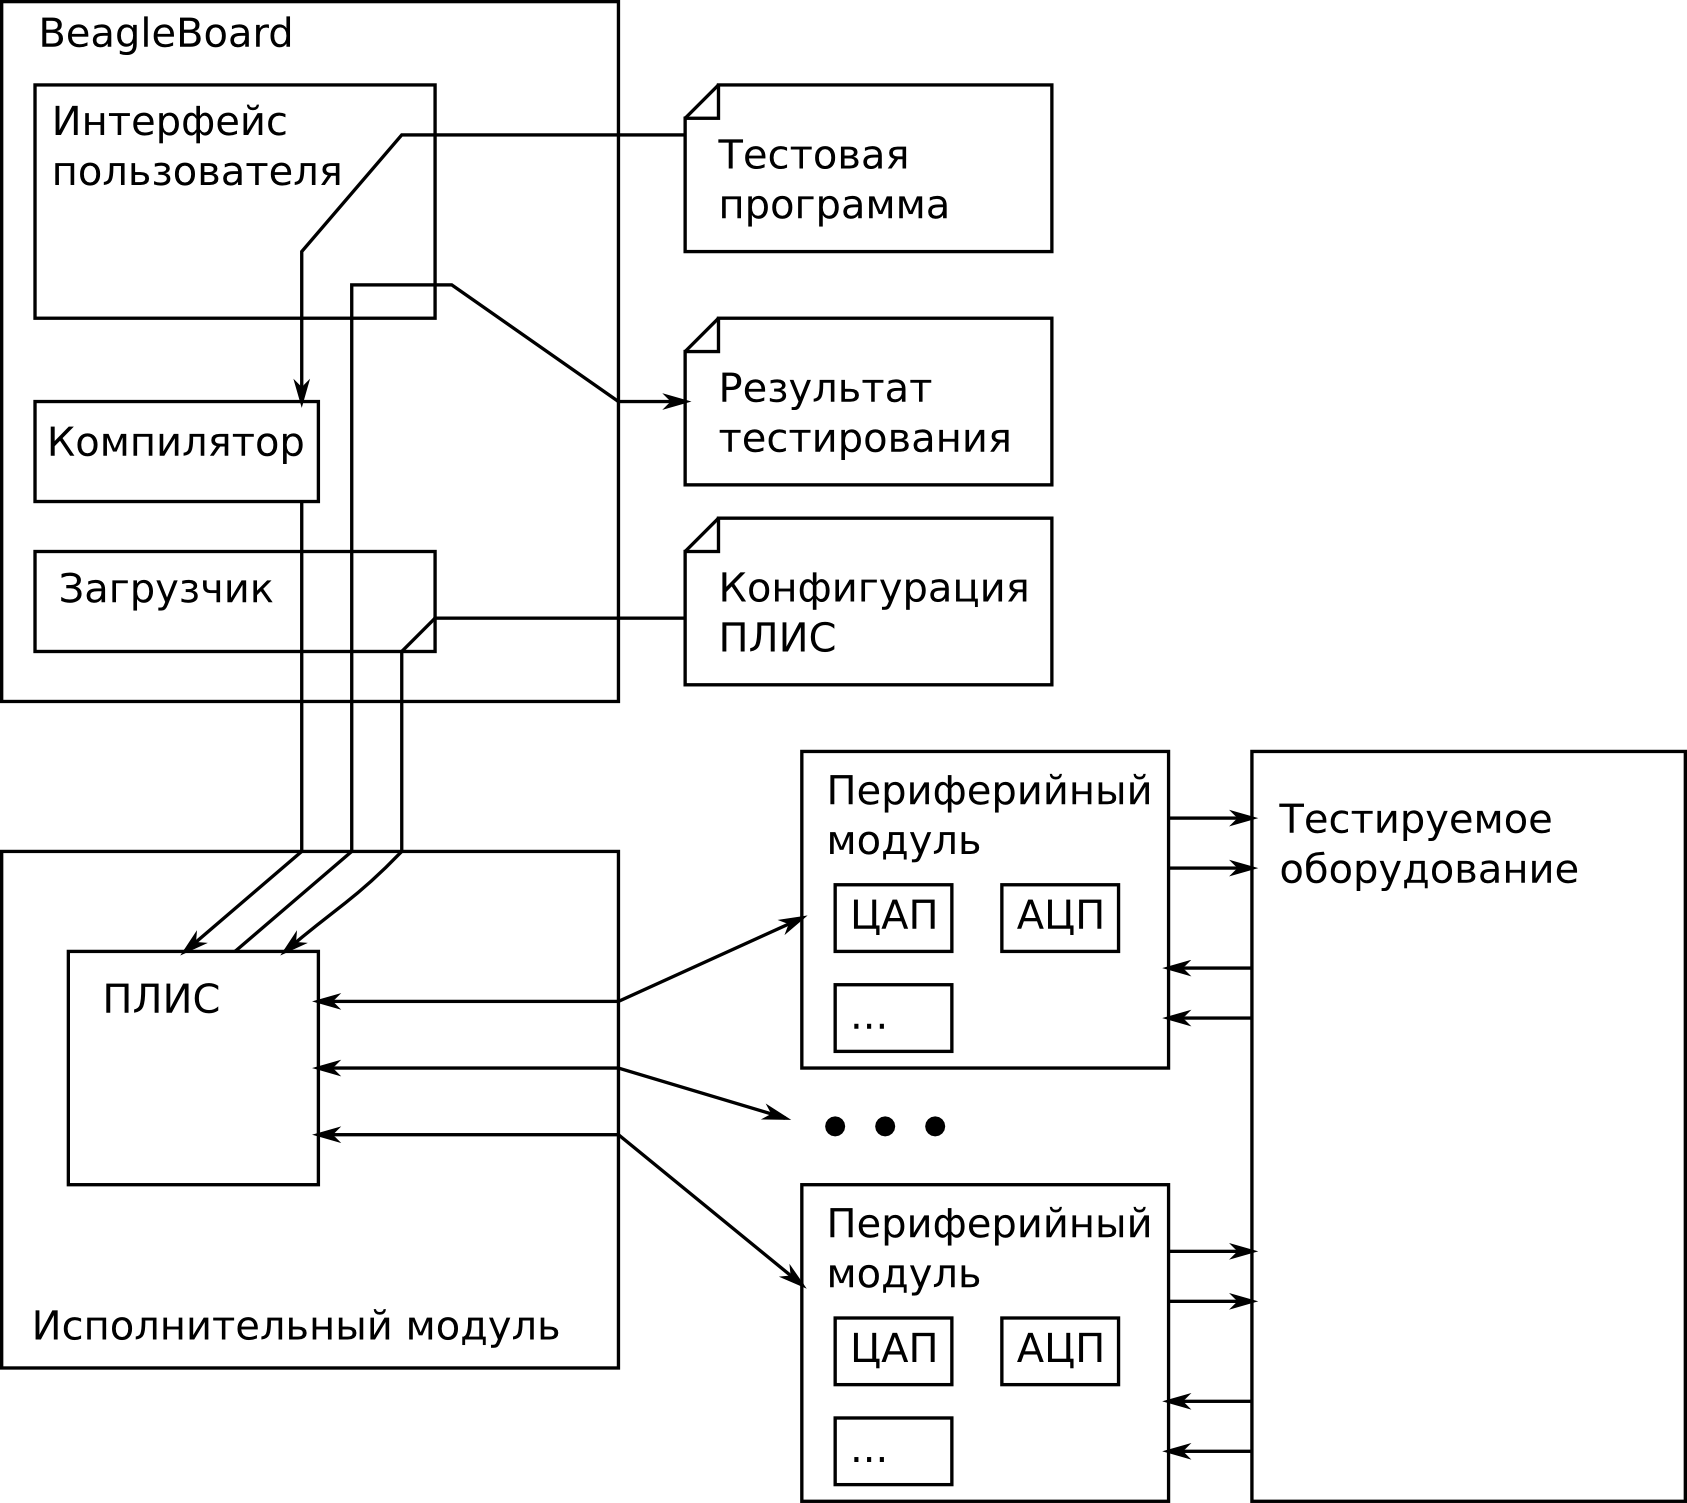
\includegraphics[width=0.95\textwidth,height=0.8\textheight,keepaspectratio]{arch.png}
\end{figure}
\end{frame}

%------------------------------------------------

\begin{frame}
\frametitle{Почему ПЛИС?}
\begin{itemize}
\item Большое число линий ввода-вывода;
\item Простота реализации системы реального времени;
\item Гибкость.
\end{itemize}
\end{frame}

%------------------------------------------------

\begin{frame}
\frametitle{Архитектура системы на кристалле}
\begin{figure}
\includegraphics[width=0.95\linewidth]{system.png}
\end{figure}
\end{frame}

%------------------------------------------------

\begin{frame}
\frametitle{Система команд процессора}
\begin{itemize}
\item SET;
\item WAIT;
\item PAUSE;
\item WIN;
\item NOP.
\end{itemize}
\end{frame}


%------------------------------------------------

\begin{frame}
\frametitle{Программное обеспечение}
\begin{enumerate}
\item Загрузчик конфигурации ПЛИС;
\item Компилятор тестовых программ;
\item Графический интерфейс пользователя.
\end{enumerate}
\end{frame}

%------------------------------------------------

\begin{frame}
\Huge{\centerline{Вопросы?}}
\end{frame}

%----------------------------------------------------------------------------------------

\end{document} 
